\documentclass[tikz,border=5pt]{standalone}
\usepackage{pgfplots}
\pgfplotsset{compat=1.18}
\usepackage{fontspec}
\setsansfont{SourceSansPro}[
  Path = /usr/local/texlive/2024/texmf-dist/fonts/opentype/adobe/sourcesanspro/,
  UprightFont = SourceSansPro-Regular.otf,
  BoldFont = SourceSansPro-Bold.otf,
  ItalicFont = SourceSansPro-RegularIt.otf,
  BoldItalicFont = SourceSansPro-BoldIt.otf,
  Scale = 1.0
]
\usetikzlibrary{positioning}
\usepackage{xcolor}
\definecolor{primaryblue}{HTML}{012169}
\definecolor{primarygold}{HTML}{B9975B}
\definecolor{highlightyellow}{HTML}{F2A900}
\definecolor{lightbg}{HTML}{E8EDF5}
\definecolor{jet}{HTML}{1A1A1A}
\definecolor{positivegreen}{HTML}{15803D}
\definecolor{negativered}{HTML}{B91C1C}
\begin{document}
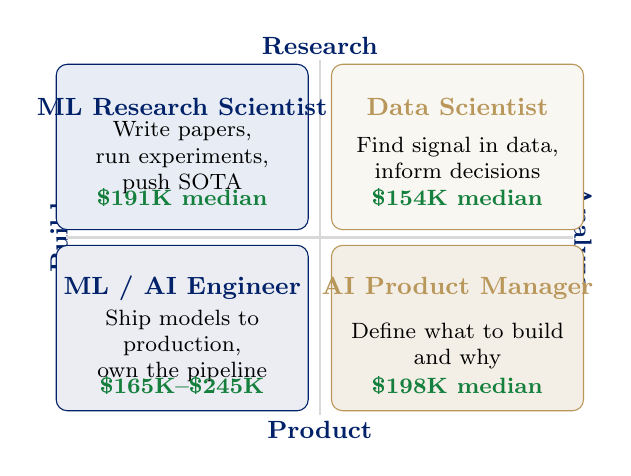
\begin{tikzpicture}[scale=0.92]
  % Axes labels
  \node[font=\small\bfseries\color{primaryblue}] at (3.5, 5.1)  {Research};
  \node[font=\small\bfseries\color{primaryblue}] at (3.5, -0.2) {Product};
  \node[font=\small\bfseries\color{primaryblue}] at (-0.1, 2.45) [rotate=90] {Build};
  \node[font=\small\bfseries\color{primaryblue}] at (7.1,  2.45) [rotate=270] {Analyze};

  % Grid lines
  \draw[gray!30, thick] (0,2.45) -- (7, 2.45);
  \draw[gray!30, thick] (3.5,0)  -- (3.5, 4.9);

  % Quadrant: Research + Build (top-left)
  \node[draw=primaryblue, fill=lightbg, rounded corners=4pt,
        minimum width=3.2cm, minimum height=2.1cm, align=center]
        at (1.6, 3.7) {};
  \node[font=\small\bfseries\color{primaryblue}, align=center]
        at (1.6, 4.25) {ML Research Scientist};
  \node[font=\footnotesize, align=center, text width=2.8cm]
        at (1.6, 3.55) {Write papers, run experiments,\\push SOTA};
  \node[font=\footnotesize\bfseries\color{positivegreen}]
        at (1.6, 3.0) {\$191K median};

  % Quadrant: Research + Analyze (top-right)
  \node[draw=primarygold, fill=primarygold!8, rounded corners=4pt,
        minimum width=3.2cm, minimum height=2.1cm, align=center]
        at (5.4, 3.7) {};
  \node[font=\small\bfseries\color{primarygold}, align=center]
        at (5.4, 4.25) {Data Scientist};
  \node[font=\footnotesize, align=center, text width=2.8cm]
        at (5.4, 3.55) {Find signal in data,\\inform decisions};
  \node[font=\footnotesize\bfseries\color{positivegreen}]
        at (5.4, 3.0) {\$154K median};

  % Quadrant: Product + Build (bottom-left)
  \node[draw=primaryblue, fill=primaryblue!8, rounded corners=4pt,
        minimum width=3.2cm, minimum height=2.1cm, align=center]
        at (1.6, 1.2) {};
  \node[font=\small\bfseries\color{primaryblue}, align=center]
        at (1.6, 1.75) {ML / AI Engineer};
  \node[font=\footnotesize, align=center, text width=2.8cm]
        at (1.6, 0.95) {Ship models to production,\\own the pipeline};
  \node[font=\footnotesize\bfseries\color{positivegreen}]
        at (1.6, 0.4) {\$165K--\$245K};

  % Quadrant: Product + Analyze (bottom-right)
  \node[draw=primarygold, fill=primarygold!15, rounded corners=4pt,
        minimum width=3.2cm, minimum height=2.1cm, align=center]
        at (5.4, 1.2) {};
  \node[font=\small\bfseries\color{primarygold}, align=center]
        at (5.4, 1.75) {AI Product Manager};
  \node[font=\footnotesize, align=center, text width=2.8cm]
        at (5.4, 0.95) {Define what to build\\and why};
  \node[font=\footnotesize\bfseries\color{positivegreen}]
        at (5.4, 0.4) {\$198K median};
\end{tikzpicture}
\end{document}
